\documentclass[12pt]{beamer}
\usepackage{../Estilos/BeamerMAF}
%Sección para el tema de beamer, con el theme, usercolortheme y sección de footers
\usetheme{CambridgeUS}
\usecolortheme{beaver}
%\useoutertheme{default}
\setbeamercovered{invisible}
% or whatever (possibly just delete it)
\setbeamertemplate{section in toc}[sections numbered]
\setbeamertemplate{subsection in toc}[subsections numbered]
\setbeamertemplate{subsection in toc}{\leavevmode\leftskip=3.2em\rlap{\hskip-2em\inserttocsectionnumber.\inserttocsubsectionnumber}\inserttocsubsection\par}
\setbeamercolor{section in toc}{fg=blue}
\setbeamercolor{subsection in toc}{fg=blue}
\setbeamercolor{frametitle}{fg=blue}
\setbeamertemplate{caption}[numbered]

\setbeamertemplate{footline}
\beamertemplatenavigationsymbolsempty
\setbeamertemplate{headline}{}


\makeatletter
\setbeamercolor{section in foot}{bg=gray!30, fg=black!90!orange}
\setbeamercolor{subsection in foot}{bg=blue!30!yellow, fg=red}
\setbeamercolor{date in foot}{bg=black, fg=white}
\setbeamertemplate{footline}
{
  \leavevmode%
  \hbox{%
  \begin{beamercolorbox}[wd=.333333\paperwidth,ht=2.25ex,dp=1ex,center]{section in foot}%
    \usebeamerfont{section in foot} \insertsection
  \end{beamercolorbox}%
  \begin{beamercolorbox}[wd=.333333\paperwidth,ht=2.25ex,dp=1ex,center]{subsection in foot}%
    \usebeamerfont{subsection in foot}  \insertsubsection
  \end{beamercolorbox}%
  \begin{beamercolorbox}[wd=.333333\paperwidth,ht=2.25ex,dp=1ex,right]{date in head/foot}%
    \usebeamerfont{date in head/foot} \insertshortdate{} \hspace*{2em}
    \insertframenumber{} / \inserttotalframenumber \hspace*{2ex} 
  \end{beamercolorbox}}%
  \vskip0pt%
}
\makeatother\newlength{\depthofsumsign}
\setlength{\depthofsumsign}{\depthof{$\sum$}}
\newcommand{\nsum}[1][1.4]{% only for \displaystyle
    \mathop{%
        \raisebox
            {-#1\depthofsumsign+1\depthofsumsign}
            {\scalebox
                {#1}
                {$\displaystyle\sum$}%
            }
    }
}
\def\scaleint#1{\vcenter{\hbox{\scaleto[3ex]{\displaystyle\int}{#1}}}}
\def\bs{\mkern-12mu}






\setbeamercolor{section in foot}{bg=deepblue, fg=white}
\setbeamercolor{subsection in foot}{bg=armygreen, fg=white}
\setbeamercolor{date in foot}{bg=goldenrod, fg=white}

\makeatletter
\setbeamertemplate{footline}
{
  \leavevmode%
  \hbox{%
  \begin{beamercolorbox}[wd=.333333\paperwidth,ht=2.25ex,dp=1ex,center]{section in foot}%
    \usebeamerfont{section in foot} \insertsection
  \end{beamercolorbox}%
  \begin{beamercolorbox}[wd=.333333\paperwidth,ht=2.25ex,dp=1ex,center]{subsection in foot}%
    \usebeamerfont{subsection in foot}  \insertsubsection
  \end{beamercolorbox}%
  \begin{beamercolorbox}[wd=.333333\paperwidth,ht=2.25ex,dp=1ex,right]{date in head/foot}%
    \usebeamerfont{date in head/foot} \insertshortdate{} \hspace*{2em}
    \insertframenumber{} / \inserttotalframenumber \hspace*{2ex} 
  \end{beamercolorbox}}%
  \vskip0pt%
}
\makeatother

\newenvironment{innerItemize}{%
  \begin{itemize}[<1->]%
}{%
  \end{itemize}%
}

\usefonttheme{serif}
\resetcounteronoverlays{saveenumi}

\date{3 de marzo de 2022}

\title{\large{Ecuaciones de la Física Matemática}}
\subtitle{Tema 2 - Primeras técnicas de solución}
\author{M. en C. Gustavo Contreras Mayén}


\begin{document}
\maketitle
\fontsize{14}{14}\selectfont
\spanishdecimal{.}

%Ref. Farlow (1993) PDE for scientists and engineers. Lesson 1 - Intro to PDE

\section{Ecuaciones diferenciales parciales}
\frame[allowframebreaks]{\tableofcontents[currentsection, hideothersubsections]}
\subsection{Introducción}

\begin{frame}
\frametitle{Las ecuaciones diferenciales}
La mayoría de los fenómenos físicos, ya sea en el dominio de la dinámica de fluidos, la electricidad, el magnetismo, la mecánica clásica o cuántica, la óptica o el flujo de calor, pueden describirse en general mediante \emph{ecuaciones diferenciales parciales} (EDP).
\end{frame}
\begin{frame}
\frametitle{Las ecuaciones diferenciales y la física}
Encontraremos que la mayoría de la física matemática se expresa con las EDP.
\\
\bigskip
\pause
Es cierto que se pueden hacer simplificaciones que reduzcan las ecuaciones en cuestión a ecuaciones diferenciales ordinarias, sin embargo, la descripción completa de estos sistemas reside en el área general de las EDP.
\end{frame}

\subsection{Definición}
\begin{frame}
\frametitle{¿Qué es una EDP}
Una ecuación diferencial parcial es una ecuación que contiene derivadas parciales.
\\
\bigskip
\pause
En contraste con las ecuaciones diferenciales ordinarias (EDO), donde la función desconocida depende solo de una variable, en las EDP, la función desconocida depende de varias variables (como la temperatura $u (x, t)$ depende tanto de la posición $x$ como del tiempo $t$).
\end{frame}
\begin{frame}
\frametitle{¿Cómo escribir una EDP?}
La representación de una derivada parcial se acostumbra utilizar la notación de Leibniz, como un cociente $\pdv*{u}{t}$, para simplificar la escritura, haremos uso de la siguiente notación tensorial, es decir, con subíndices:
\begin{align*}
u_{t} &= \pdv{u}{t} \hspace{1cm} u_{x} = \pdv{u}{x} \\[0.5em]
u_{xx} &= \pdv[2]{u}{x} \hspace{1cm} u_{xy} = \pdv[2]{u}{x}{y}
\end{align*}
\end{frame}
\begin{frame}
\frametitle{Forma general de una EDP}
La forma general de una ecuación diferencial parcial (EDP) que involucra a dos variables independientes: $x$ e $y$, está dada por:
\pause
\begin{align}
\begin{aligned}
F(x, y, \phi_{x}, \phi_{y}, \phi_{xx}, \phi_{yy}, \phi_{xy}, \phi_{xxx}, \phi_{yyy}, \ldots) = 0 \\[0.5em]
 x, y \in \Omega
\end{aligned}
\label{eq:ecuacion_B01_01}
\end{align}
donde $\Omega$ es un dominio dado, $F$ es una función con los argumentos que se indican y $\phi$ es una función arbitraria de $(x, y)$.
\end{frame}
\begin{frame}
\frametitle{La solución de una EDP}
Una solución de la ec. (\ref{eq:ecuacion_B01_01}) corresponde a la función $\phi(x, y)$ que cumple (\ref{eq:ecuacion_B01_01}) para todos los valores de $x$ e $y$.
\end{frame}
\begin{frame}
\frametitle{Dominio de las variables}
Si estamos manejando $n$ variables independientes $x_{1}, x_{2}, \ldots, x_{n}$, el dominio $\Omega$ se refiere al espacio n-dimensional que contiene una hipersuperficie $(n-1)$-dimensional.
\\
\bigskip
\pause
Una hipersuperficie de dimensión $(n-1)$ está dada por la ecuación de la forma $x_{1}^{2} + x_{2}^{2} + \ldots + x_{n}^{2} = 1$ en el espacio Euclidiano n-dimensional.
\end{frame}
\begin{frame}
\frametitle{Tipos de variables en una EDP}
Veamos de los ejemplos anteriores que la función desconocida $u$ siempre depende de más de una variable.
\\
\bigskip
\pause
La variable $u$ (que diferenciamos) se llama \textbf{variable dependiente}, mientras que aquellas con respecto a las que diferenciamos se llaman \textbf{variables independientes}.
\end{frame}
\begin{frame}
\frametitle{Tipos de variable en una EDP}
Por ejemplo, de la ecuación:
\pause
\begin{align*}
\text{\Large{$u_{t} = u_{xx}$}}
\end{align*}
la variable dependiente $u(x, t)$ es una función de dos variables independientes $x$ y $t$.
\end{frame}
\begin{frame}
\frametitle{Tipos de variable en una EDP}
Mientras que para la ecuación:
\pause
\begin{align*}
\text{\Large{$u_{t} = u_{rr} + \dfrac{1}{r} \, u_{r} + \dfrac{1}{r^{2}} \, u_{\theta \theta}$}}
\end{align*}
se tiene que $u(r, \theta, t)$ depende de las variables $r$, $\theta$ y $t$.
\end{frame}

\subsection{¿Por qué son útiles las EDP?}

\begin{frame}
\frametitle{Uso de las EDP}
La mayoría de las leyes naturales de la física, como las ecuaciones de Maxwell, \pause la ley de enfriamiento de Newton, \pause las ecuaciones de Navier-Stokes, \pause las ecuaciones de movimiento de Newton \pause y la ecuación de Schrödinger de la mecánica cuántica, entre otras.
\end{frame}
\begin{frame}
\frametitle{Uso de las EDP}
Estas ecuaciones se expresan (o pueden ser expresadas) en términos de EDP, \pause es decir, estas leyes describen los fenómenos físicos relacionando las derivadas espaciales y temporales.
\end{frame}
\begin{frame}
\frametitle{Uso de las EDP}
Las derivadas se presentan en estas ecuaciones porque las derivadas modelan cosas naturales (como velocidad, aceleración, fuerza, fricción, flujo, corriente).
\\
\bigskip
\pause
Por tanto, tenemos ecuaciones que relacionan derivadas parciales de alguna cantidad desconocida que nos gustaría encontrar.
\end{frame}

\section{¿Cómo se resuelve una EDP?}
\frame[allowframebreaks]{\tableofcontents[currentsection, hideothersubsections]}
\subsection{Técnicas de solución}

\begin{frame}
\frametitle{¿Cómo resolver una EDP?}
Esta es una buena pregunta que debemos de plantearnos.
\\
\bigskip
\pause
Resulta que hay conjunto amplio de métodos disponibles para resolver las EDP; \pause los métodos \emph{\textcolor{blue}{más importantes son los que convierten las EDP en EDO}}, ya que simplifican el manejo y su solución.
\end{frame}
\begin{frame}
\frametitle{La razón del nombre del Tema 2}
Es por esta razón que el nombre de este Tema 2 es: Primeras técnicas de solución.
\\
\bigskip
\pause
Aunque trabajamos con al menos tres técnicas, no implica que sean las únicas, sino que existen otras que se pueden ocupar dependiendo del problema que tengamos que resolver.
\end{frame}
\begin{frame}
\frametitle{Listado de técnicas}
A continuación mencionamos diez técnicas que son bastante útiles:
\pause
\setbeamercolor{item projected}{bg=blue!70!black,fg=yellow}
\setbeamertemplate{enumerate items}[circle]
\begin{enumerate}[<+->]
\item \emph{Separación de variables}. Esta técnica reduce una EDP de $n$ variables, a un sistema de $n$ EDO.
\item \emph{Transformadas integrales}. Este procedimiento reduce una EDP de $n$ variables independientes a una de $n - 1$ variables; por lo tanto, una EDP en dos variables podría cambiarse a una EDO.
\seti
\end{enumerate}
\end{frame}
\begin{frame}
\frametitle{Listado de técnicas}
\setbeamercolor{item projected}{bg=blue!70!black,fg=yellow}
\setbeamertemplate{enumerate items}[circle]
\begin{enumerate}[<+->]
\conti    
\item \emph{Cambio de coordenadas}. Este método cambia la EDP original a una EDO o bien a otra EDP (una más fácil) cambiando las coordenadas del problema (rotando el eje o transformaciones similares).
\item \emph{Transformación de la variable dependiente}. Este método transforma la variable incógnita de una EDP en una nueva incógnita que es más fácil de encontrar.
\seti
\end{enumerate}
\end{frame}
\begin{frame}
\frametitle{Listado de técnicas}
\setbeamercolor{item projected}{bg=blue!70!black,fg=yellow}
\setbeamertemplate{enumerate items}[circle]
\begin{enumerate}[<+->]
\conti    
\item \emph{Métodos numéricos}. Estos métodos cambian una EDP a un sistema de ecuaciones en diferencias que puede resolverse mediante un algoritmo con técnicas iterativas en una computadora; en muchos casos, esta es la única técnica que funcionará.
\\
\bigskip
\pause
Además de los métodos que reemplazan las EDP por ecuaciones en diferencias, existen otros métodos que intentan aproximar soluciones mediante curvas polinomiales (aproximaciones spline).
\seti
\end{enumerate}
\end{frame}
\begin{frame}
\frametitle{Listado de técnicas}
\setbeamercolor{item projected}{bg=blue!70!black,fg=yellow}
\setbeamertemplate{enumerate items}[circle]
\begin{enumerate}[<+->]
\conti    
\item \emph{Métodos de perturbación}. Este método convierte un problema no lineal en una secuencia de problemas lineales que se aproxima al no lineal.
\item \emph{Técnica impulso-respuesta}. Este procedimiento descompone las condiciones iniciales y de frontera del problema en impulsos simples y encuentra la respuesta a cada impulso. La respuesta general se encuentra luego agregando estas respuestas simples.
\seti
\end{enumerate}
\end{frame}
\begin{frame}
\frametitle{Listado de técnicas}
\setbeamercolor{item projected}{bg=blue!70!black,fg=yellow}
\setbeamertemplate{enumerate items}[circle]
\begin{enumerate}[<+->]
\conti    
\item \emph{Ecuaciones integrales}. Esta técnica cambia una EDP a una ecuación integral (una ecuación donde la incógnita está dentro de la integral). Luego, la ecuación integral se resuelve mediante varias técnicas.
\seti
\end{enumerate}
\end{frame}
\begin{frame}
\frametitle{Listado de técnicas}
\setbeamercolor{item projected}{bg=blue!70!black,fg=yellow}
\setbeamertemplate{enumerate items}[circle]
\begin{enumerate}[<+->]
\conti    
\item \emph{Métodos de cálculo de variaciones}. Estos métodos encuentran la solución a las EDP reformulando la ecuación como un problema de minimización. Resulta que el mínimo de cierta expresión (muy probablemente la expresión representará la energía total) también es la solución a la EDP.
\seti
\end{enumerate}
\end{frame}
\begin{frame}
\frametitle{Listado de técnicas}
\setbeamercolor{item projected}{bg=blue!70!black,fg=yellow}
\setbeamertemplate{enumerate items}[circle]
\begin{enumerate}[<+->]
\conti    
\item \emph{Expansión de funciones propias (eigenfunciones)}. Este método intenta encontrar la solución de una EDP como una suma infinita de funciones propias.
\\
\bigskip
\pause    
Este tipo de problemas con funciones propias se resuelven lo que se conoce como un problema de valores propios correspondiente al problema original.
\end{enumerate}
\end{frame}

\section{Tipos de EDP}
\frame[allowframebreaks]{\tableofcontents[currentsection, hideothersubsections]}
\subsection{Criterios para clasificarlas}

\begin{frame}
\frametitle{Clasificando las EDP}
Las ecuaciones diferenciales parciales se clasifican de acuerdo a ciertas características que presentan.
\\
\bigskip
\pause
La clasificación es un concepto importante porque la teoría general y \emph{los métodos de solución generalmente se aplican solo a una clase determinada} de ecuaciones.
\end{frame}
\begin{frame}
\frametitle{Criterios de clasificación}
A continuación enlistamos seis clasificaciones básicas:
\pause
\setbeamercolor{item projected}{bg=blue!70!black,fg=yellow}
\setbeamertemplate{enumerate items}[circle]
\begin{enumerate}[<+->]
\item \textbf{Orden de la EDP}. El orden de una EDP es el orden de la derivada parcial más alta, por ejemplo:
\pause
\begin{table}[H]
\centering
\begin{tabular}{l l}
\Large{$u_{t} = u_{xx}$} & es de segundo orden \\ \pause
\Large{$u_{t} = u_{x}$} & es de primer orden \\ \pause
\Large{$u_{t} = u \, u_{xxx} + \sin x$} & es de tercer orden
\end{tabular}
\end{table}
\seti
\end{enumerate}
\end{frame}
\begin{frame}
\frametitle{Criterios de clasificación}
\setbeamercolor{item projected}{bg=blue!70!black,fg=yellow}
\setbeamertemplate{enumerate items}[circle]
\begin{enumerate}[<+->]    
\conti
\item \textbf{Número de variables}. El número de variables es el número de variables independientes, por ejemplo:
\begin{table}[H]
\centering
\large
\begin{tabular}{l l}
\Large{$u_{t} = u_{xx}$} & dos variables: $x, t$ \\
\Large{$u_{t} = u_{rr} + \dfrac{1}{r} \, u_{r} + \dfrac{1}{r^{2}} \, u_{\theta \theta}$} & tres variables: $r, \theta, t$
\end{tabular}
\end{table}
\seti
\end{enumerate}
\end{frame}
\begin{frame}
\frametitle{Criterios de clasificación}
\setbeamercolor{item projected}{bg=blue!70!black,fg=yellow}
\setbeamertemplate{enumerate items}[circle]
\begin{enumerate}[<+->]    
\conti
\item \textbf{Linealidad}. Las EDP son lineales o no lineales. \pause En las lineales, la variable dependiente $u$ y todas sus derivadas aparecen de forma lineal (no se multiplican juntas ni al cuadrado, por ejemplo).
\seti
\end{enumerate}
\end{frame}
\begin{frame}
\frametitle{Linealidad en las EDP}
Más precisamente, una \emph{ecuación lineal de segundo orden en dos variables} es una ecuación de la forma:
\pause
\begin{align}
\addtolength{\fboxsep}{5pt}\boxed{ A \, u_{xx} + B \, u_{xy} + C \, u_{yy} + D \, u_{x} + E \, u_{y} + F \, u = G}
\label{eq:ecuacion_01_01}
\end{align}
donde $A, B, C, D, E, F$ y $G$ pueden ser \emph{constantes} o \emph{funciones de} $(x, y)$.
\end{frame}
\begin{frame}
\frametitle{Linealidad en las EDP}
Por ejemplo:
\pause
\begin{table}[H]
\centering
\large
\begin{tabular}{l p{1cm} l}
\Large{$e^{-t} \, u_{xx} + \sin t = u_{tt}$} & & lineal \\ \pause
\Large{$u \, u_{xx} + u_{t} = 0$} & & no lineal \\ \pause
\Large{$u_{xx} + y \, u_{yy} = 0$} & & lineal \\ \pause
\Large{$x \, u_{x} + y \, u_{y} + u^{2} = 0$} & & no lineal
\end{tabular}
\end{table}
\end{frame}
\begin{frame}
\frametitle{Criterios de clasificación}
\setbeamercolor{item projected}{bg=blue!70!black,fg=yellow}
\setbeamertemplate{enumerate items}[circle]
\begin{enumerate}[<+->]    
\conti
\item \textbf{Homogeneidad}. La ec. (\ref{eq:ecuacion_01_01}) se denomina \emph{homogénea} si el lado derecho de la igualdad $G(x, y)$ es cero para todo $x$, e $y$.
\\
\bigskip
\pause
Mientras que si $G(x, y)$ no se anula, entonces la ecuación se denomina \emph{no homogénea}.
\seti
\end{enumerate}
\end{frame}
\begin{frame}
\frametitle{Criterios de clasificación}
\setbeamercolor{item projected}{bg=blue!70!black,fg=yellow}
\setbeamertemplate{enumerate items}[circle]
\begin{enumerate}[<+->]    
\conti
\item \textbf{Tipo de coeficientes}. Si los coeficientes $A, B, C, D, E, F$ en la ec. (\ref{eq:ecuacion_01_01}) son constantes, entonces (\ref{eq:ecuacion_01_01}) tiene \emph{coeficientes constantes}, de otra manera, la ecuación tiene \emph{coeficientes variables}.
\seti
\end{enumerate}
\end{frame}
\begin{frame}
\frametitle{Criterios de clasificación}
\setbeamercolor{item projected}{bg=blue!70!black,fg=yellow}
\setbeamertemplate{enumerate items}[circle]
\begin{enumerate}[<+->]    
\conti
\item \textbf{Tres tipos de ecuaciones lineales}. Toda EDP lineal como la ec. (\ref{eq:ecuacion_01_01}) puede clasificarse como de tipo:
\pause
\begin{itemize}[<+->]
\item \large{Parabólico}.
\item \large{Hiperbólico}.
\item \large{Elíptico}.
\end{itemize}
\end{enumerate}
\end{frame}
\begin{frame}
\frametitle{Ecuaciones EDP parabólicas}
Las ecuaciones \textbf{parabólicas} describen por ejemplo el flujo de calor y procesos de difusión, además satisfacen la propiedad $B^{2} - 4 \, A \, C = 0$.
\end{frame}
\begin{frame}
\frametitle{Ecuaciones EDP hipérbólicas}
Las ecuaciones \textbf{hiperbólicas} describen sistemas que vibran así como el movimiento de las ondas, satisfacen la propiedad $B^{2} - 4 \, A \, C > 0$.
\end{frame}
\begin{frame}
\frametitle{Ecuaciones EDP elípticas}
Las ecuaciones \textbf{elípticas} describe fenómenos estacionarios y satisfacen la propiedad $B^{2} - 4 \, A \, C < 0$.
\end{frame}
\begin{frame}
\frametitle{Tipos de EDP}
Como ejemplo veamos:
\pause
\begin{table}[H]
\centering
\begin{tabular}{l l l l l}
\Large{$u_{t} = u_{xx}$} & & \large{$B^{2} - 4 \, A \, C = 0$} & & parabólica \\ \pause
\Large{$u_{tt} = u_{xx}$} & & \large{$B^{2} - 4 \, A \, C = 4$} & & hiperbólica \\ \pause
\Large{$u_{\xi \eta} = 0$} & & \large{$B^{2} - 4 \, A \, C = 1$} & & hiperbólica \\ \pause
\Large{$u_{xx} + u_{yy} = 0$} & & \large{$B^{2} - 4 \, A \, C = -4$} & & elíptica \\
\end{tabular}
\end{table}
\end{frame}
\begin{frame}
\frametitle{Tipos de EDP}
\begin{table}[H]
\centering
\begin{tabular}{l l l l l}    
\Large{$y \, u_{xx} + u_{yy} = 0$} & \large{$B^{2} {-} 4 A C {=} - 4 \, y$} & & & \\ \pause
es $\begin{cases}
    \action<+->{\mbox{elíptica para } y > 0} \\
    \action<+->{\mbox{parabólica para } y = 0} \\
    \action<+->{\mbox{hipérbolica para } y < 0} \\
    \end{cases}$ & & & & \\
\end{tabular}
\end{table}
\pause
En el caso de \emph{\textcolor{red}{coeficientes variables}}, el tipo de ecuación cambia de punto a punto.
\end{frame}


% \subsection*{Consideraciones}
% \begin{enumerate}
% \item En general, $B^{2} - 4 \, A \, C$ es una función de las variables independientes; por lo tanto, una ecuación puede cambiar de un tipo básico a otro en todo el dominio de la ecuación (aunque no es común).
% \item La ecuación lineal general (\ref{eq:ecuacion_01_01}) se escribió con variables independientes $x$ e $y$. En muchos problemas, una de las dos variables representa el tiempo, por lo tanto, se escribiría en términos de $x$ y $t$.
% \item En la figura (\ref{fig:figura_clasificacion_EDP}) se muestra un diagrama de clasificación general:
\begin{frame}
\frametitle{Clasificación general de las EDP}
\begin{figure}[H]
    \centering
    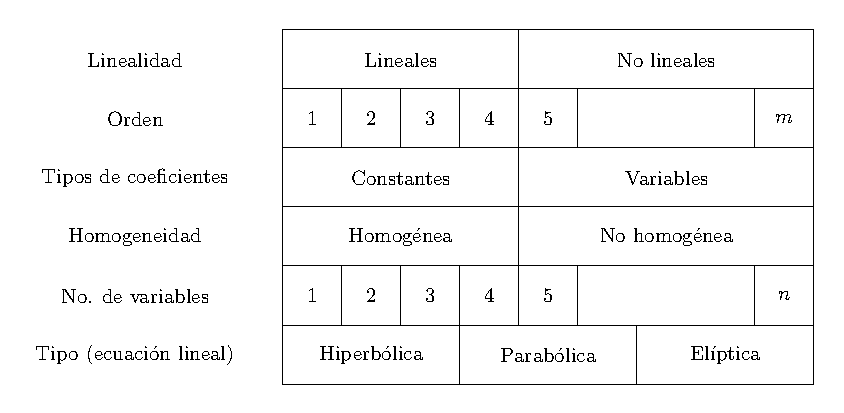
\includegraphics[scale=0.85]{Imagenes/Cuadro_Clasificacion_EDP.eps}
    % \caption{Diagrama de clasificación de EDP.}
    % \label{fig:figura_clasificacion_EDP}
\end{figure}
\end{frame}
% \end{enumerate}

% %Ref. Zamora (2012) . Notas EDP 1.1.3 Problemas asociados.

\section{Problemas asociados}
\frame[allowframebreaks]{\tableofcontents[currentsection, hideothersubsections]}
\subsection{Definición}

\begin{frame}
\frametitle{Problema asociado}
Se denomina un \emph{problema} a la EDP junto con un conjunto de condiciones dadas.
\\
\bigskip
\pause
Suponiendo una ecuación de la forma:
\begin{align}
F(x, t, u, u_{x}, u_{t}, u_{xx}, u_{xt}, u_{tt}) = 0
\label{eq:ecuacion_Z01_06}
\end{align}
es decir, una EDP de segundo orden en dos variables, se definen los distintos problemas.
\end{frame}

\subsection{Problema de Cauchy}

\begin{frame}
\frametitle{Condiciones de Cauchy}
Este problema se conoce también como \emph{problema de valores iniciales}.
\\
\bigskip
\pause
Dado el carácter de segundo orden en las derivadas respecto al tiempo $t$ de la ec. (\ref{eq:ecuacion_Z01_06}, son necesarias dos condiciones sobre la solución $u(x, t)$.
\end{frame}
\begin{frame}
\frametitle{Condiciones de Cauchy}
Estas son:
\pause
\begin{eqnarray}
u(x, 0) &= \phi (x) \label{eq:ecuacion_Z01_07} \\[0.5em] \pause
u_{t}(x, 0) &= \psi (x) \label{eq:ecuacion_Z01_08}
\end{eqnarray}
donde $\phi$ y $\psi$ son funciones dadas en el intervalo de interés, y se ha elegido el tiempo inicial $t = 0$.
\end{frame}
\begin{frame}
\frametitle{Consideración para este tipo de problemas}
Notemos que si en la EDP el orden mayor de la derivada respecto a $t$ fuese $N,$ entonces serían necesarias las derivadas parciales de $u$ respecto a $t$ desde el orden $0$ hasta el $N - 1$ evaluadas al tiempo $t = 0$ como condiciones.
\end{frame}

\subsection{Problema de Dirichlet}

\begin{frame}
\frametitle{Condiciones de Dirichlet}
Este es un tipo de problema conocido como de valores en la frontera.
\\
\bigskip
\pause
Dado el carácter de segundo orden en las derivadas respecto a la posición $x$ de la ec. (\ref{eq:ecuacion_Z01_06}), se necesitan dos condiciones sobre la solución $u(x, t)$.
\end{frame}
\begin{frame}
\frametitle{Condiciones de Dirichlet}
Suponiendo que se busca la solución para $a  \leq x \leq b$, $t \geq 0$, éstas son:
\pause
\begin{eqnarray}
u(a, t) &= f (t) \label{eq:ecuacion_Z01_09} \\[0.5em] \pause
u(b, t) &= g(t) \label{eq:ecuacion_Z01_10}
\end{eqnarray}
donde $f$ y $g$ son funciones dadas, definidas para $t \geq 0$.
\end{frame}
\begin{frame}
\frametitle{Consideraciones para este tipo de problemas}
Ahora notemos que si en la EDP el orden mayor de la derivada respecto a $x$ fuese $N$, entonces serían necesarios los valores de $u$ en $N$ distintos $x = a_{i}$ como condiciones. 
\\
\bigskip
\pause
De manera general, el problema de Dirichlet \emph{prescribe} el valor de la función incógnita, $u$, en toda la \emph{frontera} de la región de interés.
\end{frame}

\subsection{Problema de Neumann}

\begin{frame}
\frametitle{Condiciones de Neumann}
Este es otro tipo de problema de \emph{valores en la frontera}.
\\
\bigskip
\pause
 Suponiendo que se busca la solución para $a \leq x \leq b$, $t \geq 0$, las condiciones son en este caso las siguientes:
\begin{eqnarray}
u_{x}(a, t) &= f(t) \label{eq:ecuacion_Z01_11} \\[0.5em] \pause
u_{x}(b, t) &= g(t) \label{eq:ecuacion_Z01_12}
\end{eqnarray}
donde $f$ y $g$ son funciones dadas, definidas para $t \geq 0$.
\end{frame}
\begin{frame}
\frametitle{Consideración para este tipo de problemas}
Revisemos que si en la EDP el orden mayor de la derivada respecto a $x$ fuese $N$, entonces serían necesarios los valores de $u_{x}$ en $N$ distintos $x = a_{i}$ como condiciones.
\\
\bigskip
\pause
De manera general, el problema de Neumann \emph{prescribe} el valor de la derivada normal de la función incógnita, $\pdv*{u}{n}$, en toda la \emph{frontera} de la región de interés.
\end{frame}

\subsection{Problema de Robin}

\begin{frame}
\frametitle{Condiciones de Robin}
Este problema \emph{de valores en la frontera} generaliza los dos anteriores.
\\
\bigskip
\pause
Suponiendo que se busca la solución para $a \leq x \leq b$, $t \geq 0$, las condiciones son:
\pause
\begin{eqnarray}
A_{1} \, u(a, t) + B_{1} \, u_{x}(a, t) &= f(t) \label{eq:ecuacion_Z01_13} \\[0.5em] \pause
A_{2} \, u(b, t) + B_{2} \, u_{x}(b, t) &= g(t) \label{eq:ecuacion_Z01_14}
\end{eqnarray}
donde $f$ y $g$ son funciones dadas, definidas para $t \geq 0$, y $A_{1}, B_{1}, A_{2} y B_{2}$ son constantes dadas.
\end{frame}
\begin{frame}
\frametitle{Consideraciones para este tipo de problemas}
Vale la pena remarcar que si en la EDP el orden mayor de la derivada respecto a $x$ fuese $N$, entonces serían necesarios los valores de $u$ y $u_{x}$ en $N$ distintos $x = a_{i}$ como condiciones.
\end{frame}
\begin{frame}
\frametitle{Consideraciones para este tipo de problemas}
De manera general, el problema de Robin \emph{prescribe} el valor de una combinación lineal de la función incógnita $u$ y su derivada normal $\pdv*{u}{n}$ en toda la \emph{frontera} de la región de interés.
\end{frame}

\subsection{Problemas Mixtos}

\begin{frame}
\frametitle{Problemas mixtos}
Son problemas \emph{de valores en la frontera} y/o iniciales que mezclan condiciones de los anteriores.
\\
\bigskip
\pause
Suponiendo que se busca la solución para $a \leq x \leq b$, $t \geq 0$, un ejemplo sería el siguiente:
\begin{eqnarray}
A_{1} \, u(a, t) + B_{1} \, u(b, t) &= f(t) \label{eq:ecuacion_Z01_15} \\[0.5em] \pause
A_{2} \, u_{x}(a, t) + B_{2} \, u_{x}(b, t) &= g(t) (\label{eq:ecuacion_Z01_16}
\end{eqnarray}
donde $f$ y $g$ son funciones dadas, definidas para $t \geq 0$, y $A_{1}, B_{1}, A_{2}$ y $B_{2}$ son constantes dadas.
\end{frame}
\begin{frame}
\frametitle{Consideraciones para este tipo de problemas}
Notemos que si en la EDP el orden mayor de la derivada respecto a $x$ fuese $N$, entonces serían necesarios los valores de $u$ o $u_{x}$ en $N$ distintos $x = a_{i}$ como condiciones.
\end{frame}
\begin{frame}
\frametitle{Consideraciones para este tipo de problemas}
De manera general, los problemas mixtos \emph{prescriben} valores de combinaciones lineales de la función incógnita $u$ (o de su derivada normal $\pdv*{u}{n}$) evaluada en distintas partes de la \emph{frontera} de la región de interés.
\end{frame}

\section{Problemas bien definidos}
\frame[allowframebreaks]{\tableofcontents[currentsection, hideothersubsections]}
\subsection{Definición}

\begin{frame}
\frametitle{Un problema bien definido}
Se dice que un problema matemático que involucra EDP está \emph{bien definido} (o planteado) si satisface los siguientes requisitos:
\setbeamercolor{item projected}{bg=blue!70!black,fg=yellow}
\setbeamertemplate{enumerate items}[circle]
\begin{enumerate}[<+->]
\item Existencia: hay al menos una solución.
\item Unicidad: hay como máximo una solución.
\item Estabilidad: La solución depende continuamente de los datos.
\end{enumerate}
\end{frame}
\begin{frame}
\frametitle{Existencia de la solución}
El primer requisito es una condición lógica obvia, pero debemos tener en cuenta que no podemos simplemente afirmar que el problema matemático tiene una solución solo porque el problema físico tiene una solución.
\end{frame}
\begin{frame}
\frametitle{Existencia de la solución}
Bien podemos estar desarrollando erróneamente un modelo matemático, \pause digamos, que consiste en una EDP cuya solución puede no existir en absoluto.
\end{frame}
\begin{frame}
\frametitle{Unicidad de la solución}
Lo mismo puede decirse del requisito de unicidad.
\\
\bigskip
\pause
Para reflejar realmente el problema físico que tiene una solución única, \pause el problema matemático debe tener una solución única. \pause Para problemas físicos, no es suficiente saber que el problema tiene una solución única.
\end{frame}
\begin{frame}
\frametitle{Estabilidad de la solución}
Por lo tanto, el último requisito no solo es útil sino también esencial.
\\
\bigskip
\pause
Para que la solución tenga importancia física, \pause un pequeño cambio en los datos iniciales debe producir un pequeño cambio en la solución.
\end{frame}
\begin{frame}
\frametitle{Estabilidad de la solución}
Los datos de un problema físico se obtienen \break \hfill normalmente de experimentos y se aproximan para resolver el problema por métodos numéricos o aproximados.
\\
\bigskip
\pause
Es fundamental saber que el proceso de hacer una aproximación a los datos produce solo un pequeño cambio en la solución.
\end{frame}
\end{document}